% Options for packages loaded elsewhere
\PassOptionsToPackage{unicode}{hyperref}
\PassOptionsToPackage{hyphens}{url}
\PassOptionsToPackage{dvipsnames,svgnames,x11names}{xcolor}
%
\documentclass[
]{report}

\usepackage{amsmath,amssymb}
\usepackage{iftex}
\ifPDFTeX
  \usepackage[T1]{fontenc}
  \usepackage[utf8]{inputenc}
  \usepackage{textcomp} % provide euro and other symbols
\else % if luatex or xetex
  \usepackage{unicode-math}
  \defaultfontfeatures{Scale=MatchLowercase}
  \defaultfontfeatures[\rmfamily]{Ligatures=TeX,Scale=1}
\fi
\usepackage{lmodern}
\ifPDFTeX\else  
    % xetex/luatex font selection
\fi
% Use upquote if available, for straight quotes in verbatim environments
\IfFileExists{upquote.sty}{\usepackage{upquote}}{}
\IfFileExists{microtype.sty}{% use microtype if available
  \usepackage[]{microtype}
  \UseMicrotypeSet[protrusion]{basicmath} % disable protrusion for tt fonts
}{}
\makeatletter
\@ifundefined{KOMAClassName}{% if non-KOMA class
  \IfFileExists{parskip.sty}{%
    \usepackage{parskip}
  }{% else
    \setlength{\parindent}{0pt}
    \setlength{\parskip}{6pt plus 2pt minus 1pt}}
}{% if KOMA class
  \KOMAoptions{parskip=half}}
\makeatother
\usepackage{xcolor}
\setlength{\emergencystretch}{3em} % prevent overfull lines
\setcounter{secnumdepth}{-\maxdimen} % remove section numbering
% Make \paragraph and \subparagraph free-standing
\ifx\paragraph\undefined\else
  \let\oldparagraph\paragraph
  \renewcommand{\paragraph}[1]{\oldparagraph{#1}\mbox{}}
\fi
\ifx\subparagraph\undefined\else
  \let\oldsubparagraph\subparagraph
  \renewcommand{\subparagraph}[1]{\oldsubparagraph{#1}\mbox{}}
\fi


\providecommand{\tightlist}{%
  \setlength{\itemsep}{0pt}\setlength{\parskip}{0pt}}\usepackage{longtable,booktabs,array}
\usepackage{calc} % for calculating minipage widths
% Correct order of tables after \paragraph or \subparagraph
\usepackage{etoolbox}
\makeatletter
\patchcmd\longtable{\par}{\if@noskipsec\mbox{}\fi\par}{}{}
\makeatother
% Allow footnotes in longtable head/foot
\IfFileExists{footnotehyper.sty}{\usepackage{footnotehyper}}{\usepackage{footnote}}
\makesavenoteenv{longtable}
\usepackage{graphicx}
\makeatletter
\def\maxwidth{\ifdim\Gin@nat@width>\linewidth\linewidth\else\Gin@nat@width\fi}
\def\maxheight{\ifdim\Gin@nat@height>\textheight\textheight\else\Gin@nat@height\fi}
\makeatother
% Scale images if necessary, so that they will not overflow the page
% margins by default, and it is still possible to overwrite the defaults
% using explicit options in \includegraphics[width, height, ...]{}
\setkeys{Gin}{width=\maxwidth,height=\maxheight,keepaspectratio}
% Set default figure placement to htbp
\makeatletter
\def\fps@figure{htbp}
\makeatother

\makeatletter
\@ifpackageloaded{caption}{}{\usepackage{caption}}
\AtBeginDocument{%
\ifdefined\contentsname
  \renewcommand*\contentsname{Table of contents}
\else
  \newcommand\contentsname{Table of contents}
\fi
\ifdefined\listfigurename
  \renewcommand*\listfigurename{List of Figures}
\else
  \newcommand\listfigurename{List of Figures}
\fi
\ifdefined\listtablename
  \renewcommand*\listtablename{List of Tables}
\else
  \newcommand\listtablename{List of Tables}
\fi
\ifdefined\figurename
  \renewcommand*\figurename{Figure}
\else
  \newcommand\figurename{Figure}
\fi
\ifdefined\tablename
  \renewcommand*\tablename{Table}
\else
  \newcommand\tablename{Table}
\fi
}
\@ifpackageloaded{float}{}{\usepackage{float}}
\floatstyle{ruled}
\@ifundefined{c@chapter}{\newfloat{codelisting}{h}{lop}}{\newfloat{codelisting}{h}{lop}[chapter]}
\floatname{codelisting}{Listing}
\newcommand*\listoflistings{\listof{codelisting}{List of Listings}}
\makeatother
\makeatletter
\makeatother
\makeatletter
\@ifpackageloaded{caption}{}{\usepackage{caption}}
\@ifpackageloaded{subcaption}{}{\usepackage{subcaption}}
\makeatother
\ifLuaTeX
  \usepackage{selnolig}  % disable illegal ligatures
\fi
\usepackage{bookmark}

\IfFileExists{xurl.sty}{\usepackage{xurl}}{} % add URL line breaks if available
\urlstyle{same} % disable monospaced font for URLs
\hypersetup{
  pdftitle={Accelerators},
  colorlinks=true,
  linkcolor={blue},
  filecolor={Maroon},
  citecolor={Blue},
  urlcolor={Blue},
  pdfcreator={LaTeX via pandoc}}

\title{Accelerators}
\author{}
\date{2024-02-13}

\begin{document}
\maketitle

XXX: This chapter is a super-early WIP

Compute accelerators are the workhorses of the ML training. At the
beginning there were just GPUs. But now there are also TPUs, IPUs,
FPGAs, HPUs, QPUs, RDUs and more are being invented.

There exist two main ML workloads - training and inference. There is
also the finetuning workload which is usually the same as training,
unless a much lighter
\href{https://arxiv.org/abs/2106.09685}{LORA-style} finetuning is
performed. The latter requires significantly fewer resources and time
than normal finetuning.

In language models during inference the generation is performed in a
sequence - one token at a time. So it has to repeat the same
\texttt{forward} call thousands of times one smallish \texttt{matmul}
(matrix multiplication or GEMM) at a time. And this can be done on
either an accelerator, like GPU, or some of the most recent CPUs, that
can handle inference quite efficiently.

During training the whole sequence length is processed in one huge
\texttt{matmul} operation. So if the sequence length is 4k long, the
training of the same model will require a compute unit that can handle
4k times more operations than inference and do it fast. Accelerators
excel at this task. In fact the larger the matrices they have to
multiply, the more efficient the compute.

The other computational difference is that while both training and
inference have to perform the same total amount of \texttt{matmul}s in
the \texttt{forward} pass, in the \texttt{backward} pass, which is only
done for training, an additional 2x times of \texttt{matmul}s is done to
calculate the gradients with regards to inputs and weights. And an
additional \texttt{forward} is performed if activations recomputation is
used. Therefore the training process requires at 3-4x more
\texttt{matmul}s than inference.

\section{Subsections}\label{subsections}

\begin{itemize}
\tightlist
\item
  \href{nvidia/debug.md}{Troubleshooting NVIDIA GPUs}
\end{itemize}

\section{Bird's eye view on the high end accelerator
reality}\label{birds-eye-view-on-the-high-end-accelerator-reality}

While this might be changing in the future, unlike the consumer GPU
market, as of this writing there aren't that many high end accelerators,
and if you rent on the cloud, most providers will have more or less the
same few GPUs to offer.

GPUs: - As of today, ML clouds/HPCs started transitioning from NVIDIA
A100s to H100s and this is going to take some months due to the usual
shortage of NVIDIA GPUs. - AMD's MI250 started popping up here and
there, but it's unclear when it'll be easy to access those. From a
recent discussion with an AMD representative MI300 is not planned to be
in general availability until some time in 2025, though some HPCs
already plan to get them some time in 2024.

HPU: - Intel's Gaudi2 are starting to slowly emerge on Intel's cloud

IPU: - And there is Graphcore with their IPU offering. You can try these
out in \href{https://www.paperspace.com/graphcore}{Paperspace} through
their cloud notebooks.

TPU: - Google's TPUs are, of course, available but they aren't the most
desirable accelerators because you can only rent them, and the software
isn't quite easily convertible between GPUs and TPUs, and so many
(most?) developers remain in the GPU land, since they don't want to be
locked into a hardware which is a Google monopoly.

Pods and racks: - Cerebras' WaferScale Engine (WSE) - SambaNova's
DataScale - dozens of different pod and rack configs that compose the
aforementioned GPUs with super-fast interconnects.

That's about it as Q4-2023.

\section{Glossary}\label{glossary}

\begin{itemize}
\tightlist
\item
  CPU: Central Processing Unit
\item
  FPGA: Field Programmable Gate Arrays
\item
  GPU: Graphics Processing Unit
\item
  HBM: High Bandwidth Memory
\item
  HPC: High-performance Computing
\item
  HPU: Habana Gaudi AI Processor Unit
\item
  IPU: Intelligence Processing Unit
\item
  MME: Matrix Multiplication Engine
\item
  QPU: Quantum Processing Unit
\item
  RDU: Reconfigurable Dataflow Unit
\item
  TPU: Tensor Processing Unit
\end{itemize}

\section{The most important thing to
understand}\label{the-most-important-thing-to-understand}

I will make the following statement multiple times in this book - and
that it's not enough to buy/rent the most expensive accelerators and
expect a high return on investment (ROI).

The two metrics for a high ROI for ML training are: 1. the speed at
which the training will finish, because if the training takes 2-3x
longer than planned, your model could become irrelevant before it was
released - time is everything in the current super-competitive ML
market. 2. the total \$\$ spent to train the model, because if the
training takes 2-3x longer than planned, you will end up spending 2-3x
times more.

Unless the rest of the purchased/rented hardware isn't chosen carefully
to match the required workload chances are very high that the
accelerators will idle a lot and both time and \$\$ will be lost. The
most critical component is \href{../../network}{network}, then
\href{../../storage/}{storage}, and the least critical ones are
(\href{../cpu}{CPU} and \href{../cpu-memory}{CPU memory}).

If the compute is rented one usually doesn't have the freedom to choose
- the hardware is either set in stone or some components might be
replaceable but with not too many choices. Thus there are times when the
chosen cloud provider doesn't provide a sufficiently well matched
hardware, in which case it's best to seek out a different provider.

If you purchase your servers then I recommend to perform a very indepth
due diligence before buying.

Besides hardware, you, of course, need software that can efficiently
deploy the hardware.

We will discuss both the hardware and the software aspects in various
chapters of this book. You may want to start
\href{../../training/performance}{here} and
\href{../../training/model-parallelism}{here}.

\section{What Accelerator characteristics do we care
for}\label{what-accelerator-characteristics-do-we-care-for}

Let's use the NVIDIA A100 spec as a reference point in the following
sections.

\begin{figure}[H]

{\centering 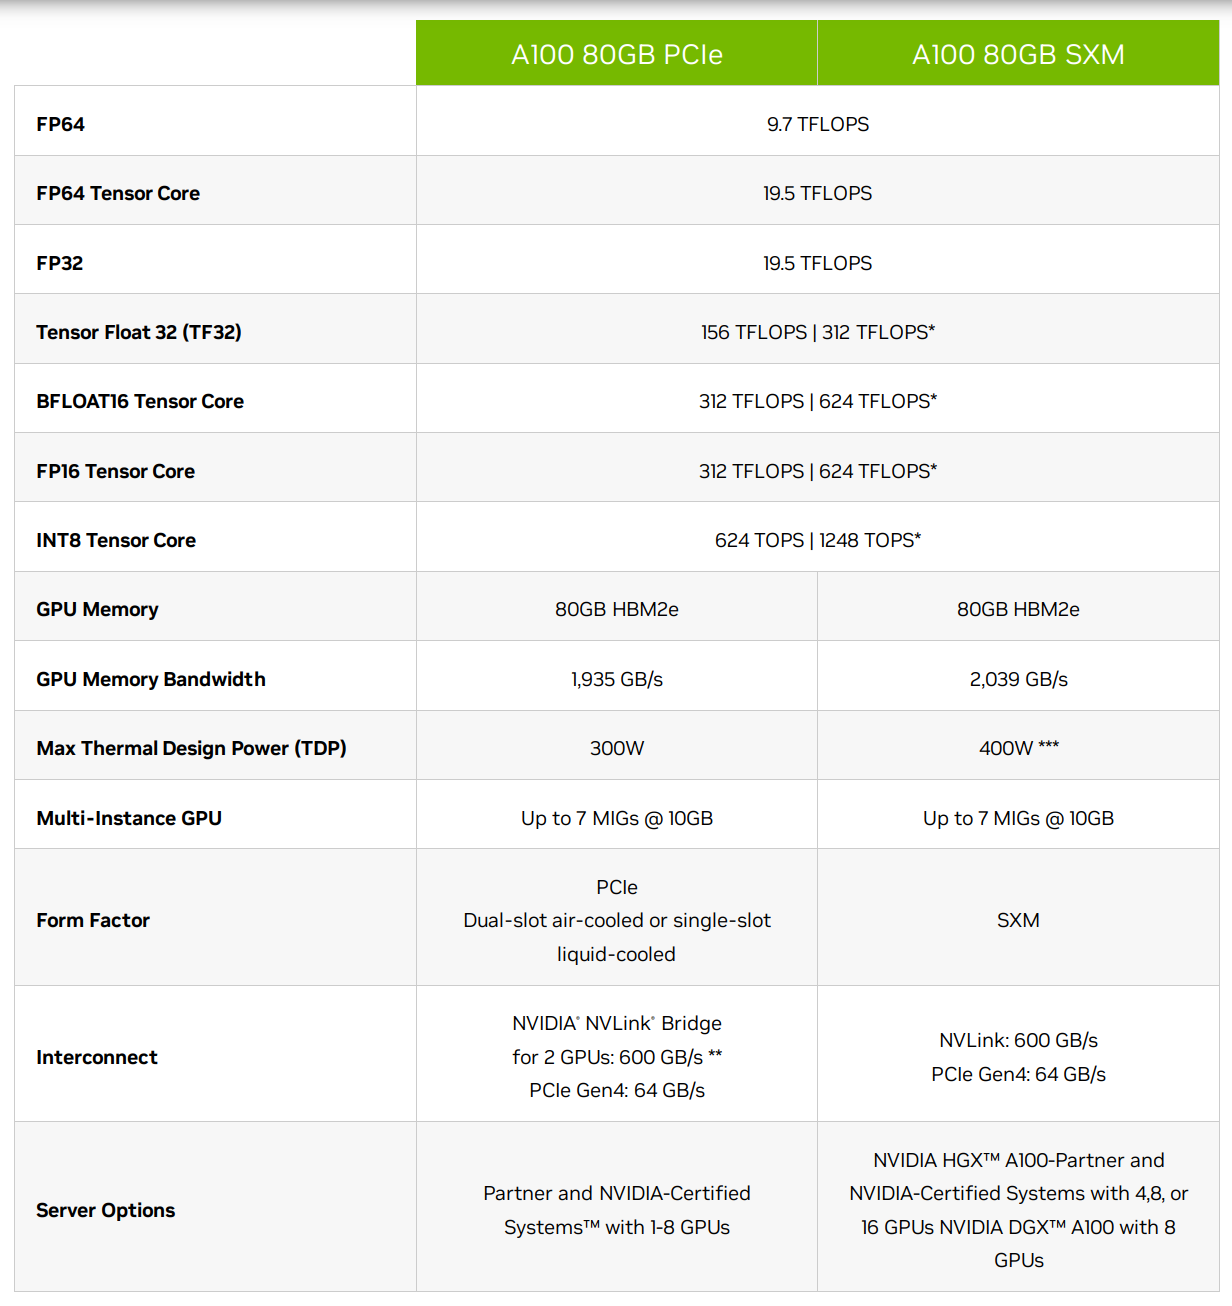
\includegraphics{images/nvidia-a100-spec.png}

}

\caption{nvidia-a100-spec}

\end{figure}%

\href{https://www.nvidia.com/en-us/data-center/a100/}{source}

\subsection{TFLOPS}\label{tflops}

As mentioned earlier most of the work that ML training and inference do
is matrix multiplication. If you remember your algebra matrix
multiplication is made of many multiplications followed by summation.
Each of these computations can be counted and define how many of these
operations can be performed by the chip in a single seconds.

This is one of the key characteristics that the accelerators are judged
by. The term TFLOPS defines how many trillions of
FloatingPointOperations the chip can perform in a second. The more the
better. There is a different definition for different data types. For
example, here are a few entries for A100:

\begin{longtable}[]{@{}lrr@{}}
\toprule\noalign{}
Data type & TFLOPS & w/ Sparsity \\
\midrule\noalign{}
\endhead
\bottomrule\noalign{}
\endlastfoot
FP32 & 19.5 & n/a \\
Tensor Float 32 (TF32) & 156 & 312 \\
BFLOAT16 Tensor Core & 312 & 624 \\
FP16 Tensor Core & 312 & 624 \\
INT8 Tensor Core & 624 & 1248 \\
\end{longtable}

footnote: INT8 is measured in TeraOperations as it's not a floating
operation.

footnote: the term FLOPS could mean either the total number of
FloatingPointOperations, e.g.~when counting how many FLOPS a single
Transformer iteration takes, and it could also mean
FloatingPointOperations per second - so watch out for the context. When
you read an accelerator spec it's almost always a per second definition.
When model architectures are discussed it's usually just the total
number of FloatingPointOperations.

So you can see that int8 is 2x faster than bf16 which in turn is 2x
faster than tf32.

Moreover, the TFLOPs depend on the matrices size as can be seen from
this table:

\begin{figure}[H]

{\centering 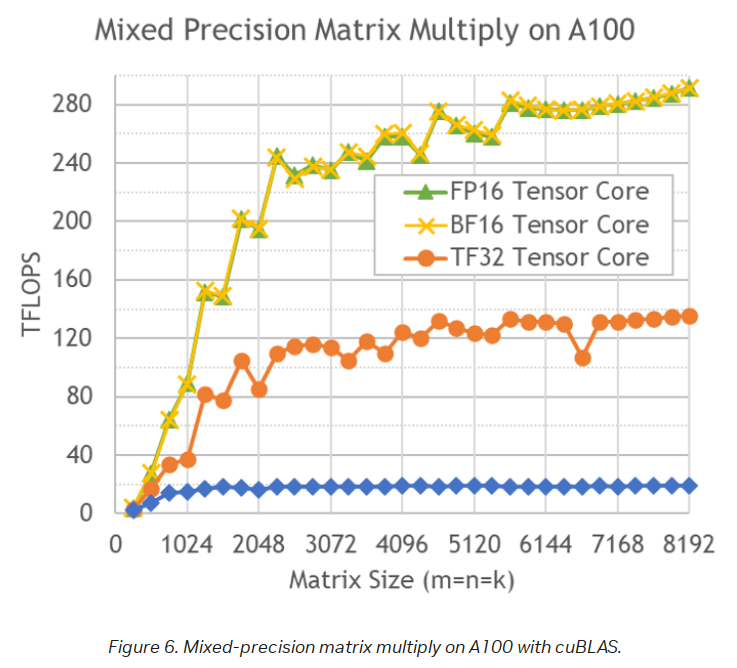
\includegraphics{images/nvidia-a100-matmul-tflops.png}

}

\caption{nvidia-a100-matmul-tflops}

\end{figure}%

\href{https://developer.nvidia.com/blog/cuda-11-features-revealed/}{source}

As you can see the difference in performance is non-linear due to
\href{https://docs.nvidia.com/deeplearning/performance/dl-performance-matrix-multiplication/index.html\#dim-quantization}{the
tile and wave quantization effects}.

Let's look at the TFLOPS specs across the high end accelerators:

\begin{longtable}[]{@{}lrrrr@{}}
\toprule\noalign{}
Accelerator / TFLOPS & fp32 & fp16 & fp8 & int8 \\
\midrule\noalign{}
\endhead
\bottomrule\noalign{}
\endlastfoot
NVIDIA A100 SXM & 19.5 & 312 & 624 & 624 \\
AMD MI250 & 45.3 & 362 & X & 362 \\
AMD MI250X & 47.9 & 383 & X & 383 \\
& & & & \\
NVIDIA H100 SXM & 67.0 & 989 & 1979 & 1979 \\
NVIDIA H100 PCIe & 51.0 & 756 & 1513 & 1513 \\
NVIDIA H100 dual NVL & 134.0 & 989 & 3958 & 3958 \\
AMD MI300 & ? & ? & ? & ? \\
& & & & \\
\end{longtable}

\begin{itemize}
\tightlist
\item
  Intel Gaudi2 doesn't plan to publish TFLOPS specs as of this writing
\end{itemize}

\subsubsection{Achievable peak TFLOPS}\label{achievable-peak-tflops}

The problem with the advertised peak TFLOPS is that they are
\textbf{very} theoretical and can't be achieved in practice even if all
the perfect conditions have been provided. Each accelerator has its own
realistic TFLOPS which is not advertised and there are anecdotal
community reports that do their best to find the actual best value, but
I'm yet to find any official reports.

If you find solid reports (papers?) showing the actual TFLOPS one can
expect from one or more of the high end accelerators discussed in this
chapter please kindly submit a PR with this information. The key is to
have a reference to a source that the reader can validate the proposed
information with.

To provide a numerical sense to what I'm talking about is let's take
A100 with its 312 TFLOPS bf16 peak performance in the specs of this
card. Until the invent of FlashAttention it was known that 150TFLOPS was
close to the highest one could get for half precision mixed precision,
with FlashAttention, it's around 180TFLOPS. This is, of course, measured
for training LLMs where the network and IO are involved which create
additional overheads. So here the peak performance probably lays
somewhere between 200 and 300 TFLOPS.

It should be possible to calculate the actual peak TFLOPS by doing a
perfectly aligned max-size matrices \texttt{matmul} measured on a single
accelerator.

XXX: write a small program to do exactly dynamically figuring out the
perfect shapes based on
\href{https://docs.nvidia.com/deeplearning/performance/dl-performance-matrix-multiplication/index.html\#dim-quantization}{the
tile and wave quantization effects} and max sizes (how?) so that the
benchmark isn't hardcoded to a particular accelerator.

\subsection{Accelerator memory size and
speed}\label{accelerator-memory-size-and-speed}

Typically the more on-chip memory the accelerator has the better. At any
given time usually most of the model weights aren't being used as they
wait for their turn to be processed and thus large memory allows more of
the model to be on the accelerator memory and immediately available for
access and update. When there is not enough memory, sometimes the model
has to be split across multiple accelerators, or offloaded to CPU and/or
disk.

Current high end accelerators (some aren't GA yet):

\begin{longtable}[]{@{}lrlr@{}}
\toprule\noalign{}
Accelerator & Memory in GBs & Type & Speed in TB/s \\
\midrule\noalign{}
\endhead
\bottomrule\noalign{}
\endlastfoot
NVIDIA A100 SXM & 80 & HBM2e & 2 \\
NVIDIA H100 SXM & 80 & HBM3 & 3.35 \\
NVIDIA H100 PCIe & 80 & HBM3 & 2 \\
NVIDIA H100 dual NVL & 188 & HBM3 & 7.8 \\
AMD MI250 & 128 & HBM2e & 3.28 \\
AMD MI250X & 128 & HBM2e & 3.28 \\
AMD MI300 & 192 & HBM3 & \\
& & & \\
\end{longtable}

\begin{itemize}
\tightlist
\item
  XXX: add other accelerators
\end{itemize}

Memory speed is, of course, very important since if it's not fast enough
than the compute ends up idling waiting for the data to be moved to and
from the memory.

The GPUs use
\href{https://en.wikipedia.org/wiki/High_Bandwidth_Memory}{High
Bandwidth Memory} (HBM) which is a 3D version of SDRAM memory. For
example, A100-SXM comes with HBM2 at 1.6TB/sec, and H100-SXM comes with
HBM3 at 3.35TB/s.

\subsection{Heat}\label{heat}

This is of interest when you buy your own hardware, when you rent on the
cloud the provider hopefully takes care of adequate cooling.

The only important practical understanding for heat is that if the
accelerators aren't kept cool they will throttle their compute clock and
slow everything down (and could even crash sometimes, albeit throttling
is supposed to prevent that).

\section{High end accelerators for LLM/VLM
workloads}\label{high-end-accelerators-for-llmvlm-workloads}

\subsection{Cloud and in-house
accelerators}\label{cloud-and-in-house-accelerators}

Most common accelerators that can be either rented on compute clouds or
purchased:

NVIDIA: -
\href{https://www.nvidia.com/en-us/data-center/a100/\#specifications}{A100}
- huge availability but already getting outdated. -
\href{https://www.nvidia.com/en-us/data-center/h100}{H100} - 2-3x faster
than A100 (half precision), 6x faster for fp8, slowly emerging on all
major clouds. -
\href{https://www.nvidia.com/en-us/data-center/grace-hopper-superchip/}{GH200}
- 2 chips on one card - (1) H100 w/ 96GB HBM3 or 144GB HBM3e + (2) Grace
CPU w/ 624GB RAM - availability is unknown.

AMD: -
\href{https://www.amd.com/en/products/accelerators/instinct/mi200/mi250.html}{MI250}
\textasciitilde= A100 - very few clouds have them - MI300
\textasciitilde= H100 - don't expect until late-2024 or even 2025 to be
GA

Intel: - \href{https://habana.ai/products/gaudi2/}{Gaudi2}
\textasciitilde= H100 - Currently there is a very low availability on
\href{https://cloud.google.com}{cloud.google.com} with a long waiting
list which supposedly should be reduced in Q1-2024. AWS has the older
Gaudi1 via \href{https://aws.amazon.com/ec2/instance-types/dl1/}{DL1
instances}.

Graphcore: - \href{https://www.graphcore.ai/products/ipu}{IPU} -
available via \href{https://www.paperspace.com/graphcore}{Paperspace}

SambaNova: - \href{https://sambanova.ai/products/datascale/}{DataScale
SN30}

\subsection{In-house accelerator
clusters}\label{in-house-accelerator-clusters}

Cerebras: - \href{https://www.cerebras.net/product-cluster/}{clusters} -
\href{https://www.cerebras.net/product-system/}{systems} based on
WaferScale Engine (WSE).

\subsection{Cloud-only solutions}\label{cloud-only-solutions}

These can be only used via clouds:

Google - \href{https://cloud.google.com/tpu}{TPUs} - lock-in, can't
switch to another vendor like NVIDIA -\textgreater{} AMD

Cerebras: - \href{https://www.cerebras.net/product-cloud/}{Cloud}

\subsection{Prices}\label{prices}

Remember that the advertised prices are almost always open to
negotiations as long as you're willing to buy/rent in bulk and if
renting then for a long time (i.e.~years!). When do you will discover
that the actual price that you end up paying could be many times less
than the original public price. Some cloud providers already include the
discount as you choose a longer commitment on their website, but it's
always the best to negotiate directly with their sales team. In addition
or instead of a \$\$-discount you could be offered some useful
features/upgrades for free.

For the baseline prices it should be easy to find a few good sites that
provide an up-to-date public price comparisons across clouds - just
search for something like
\href{https://www.google.com/search?q=cloud+gpu+pricing+comparison}{cloud
gpu pricing comparison}.

\section{Accelerators in detail}\label{accelerators-in-detail}

\subsection{NVIDIA}\label{nvidia}

Abbreviations:

\begin{itemize}
\tightlist
\item
  CUDA: Compute Unified Device Architecture (proprietary to NVIDIA)
\end{itemize}

NVIDIA-specific key GPU characteristics: - CUDA Cores - similar to CPU
cores, but unlike CPUs that typically have 10-100 powerful cores, CUDA
Cores are weaker and come in thousands and allow to perform massive
general purpose computations (parallelization). Like CPU cores CUDA
Cores perform a single operation in each clock cycle. - Tensor Cores -
special compute units that are designed specifically to perform fast
multiplication and addition operations like matrix multiplication. These
perform multiple operations in each clock cycle. They can execute
extremely fast computations on low or mixed precision data types with
some loss (fp16, bf16, tf32, fp8, etc.). These cores are specifically
designed for ML workloads. - Streaming Multiprocessors (SM) are clusters
of CUDA Cores, Tensor Cores and other components.

For example, A100-80GB has:

\begin{itemize}
\tightlist
\item
  6912 CUDA Cores
\item
  432 Tensor Cores (Gen 3)
\item
  108 Streaming Multiprocessors (SM)
\end{itemize}

\subsection{AMD}\label{amd}

AMD-specific key GPU characteristics: - Stream Processors - are similar
in functionality to CUDA Cores - that is these are the parallel
computation units. But they aren't the same, so one can't compare 2 gpus
by just comparing the number of CUDA Cores vs the number of Stream
Processors. - Compute Units - are clusters of Stream Processors and
other components

for example, AMD MI250 has: - 13,312 Stream Processors - 208 Compute
Units

\subsection{Intel Gaudi2}\label{intel-gaudi2}

\href{https://docs.habana.ai/en/latest/Gaudi_Overview/Gaudi_Architecture.html}{Architecture}

\begin{itemize}
\tightlist
\item
  24x 100 Gigabit Ethernet (RoCEv2) integrated on chip - 21 of which are
  used for intra-node and 3 for inter-node (so \texttt{21*8=168} cards
  for intra-node (262.5GBps per GPU), and \texttt{3*8=24} cards for
  inter-node (2.4Tbps between nodes)
\item
  96GB HBM2E memory on board w/2.45 TBps bandwidth per chip, for a total
  of 768GB per node
\end{itemize}

A server/node is built from 8 GPUs, which can then be expanded with
racks of those servers.

There are no official TFLOPS information published (and from talking to
an Intel representative they have no intention to publish any.) They
publish the {[}following
benchmarks{]}(https://developer.habana.ai/resources/habana-models-performance/
but I'm not sure how these can be used to compare this compute to other
providers.

Comparison: supposedly Gaudi2 competes with NVIDIA H100

\section{API}\label{api}

\subsection{NVIDIA}\label{nvidia-1}

uses CUDA

\subsection{AMD}\label{amd-1}

uses ROCm

\subsection{Intel Gaudi}\label{intel-gaudi}

The API is via \href{https://habana.ai/training-software/}{Habana
SynapseAI® SDK} which supports PyTorch and TensorFlow.

Useful integrations: -
\href{https://github.com/huggingface/optimum-habana}{HF Optimum Habana}
which also includes -
\href{https://github.com/microsoft/DeepSpeed}{DeepSpeed} integration.

\section{Apples-to-apples Comparison}\label{apples-to-apples-comparison}

It's very difficult to compare specs of different offerings since
marketing tricks get deployed pretty much by all competitors so that one
can't compare 2 sets of specs and know the actual difference.

\begin{itemize}
\item
  \href{https://mlcommons.org/en/}{MLPerf via MLCommons} publishes
  various hardware benchmarks that measure training, inference, storage
  and other tasks' performance. For example, here is the most recent as
  of this writing
  \href{https://mlcommons.org/en/training-normal-30/}{training v3.0} and
  \href{https://mlcommons.org/en/inference-datacenter-31/}{inference
  v3.1} results.

  Except I have no idea how to make use of it - it's close to impossible
  to make sense of or control the view. This is a great intention lost
  in over-engineering and not thinking about how the user will benefit
  from it, IMHO. For example, I don't care about CV data, I only want to
  quickly see the LLM rows, but I can't do it. And then the comparisons
  are still not apples to apples so how can you possibly make sense of
  which hardware is better I don't know.
\end{itemize}

\section{Power and Cooling}\label{power-and-cooling}

It is most likely that you're renting your accelerator nodes and someone
else is responsible for ensuring they function properly, but if you own
the accelerators you do need to know how to supply a sufficient power
and adequate cooling.

\subsection{Power}\label{power}

Some high end consumer GPU cards have 2 and sometimes 3 PCI-E 8-Pin
power sockets. Make sure you have as many independent 12V PCI-E 8-Pin
cables plugged into the card as there are sockets. Do not use the 2
splits at one end of the same cable (also known as pigtail cable). That
is if you have 2 sockets on the GPU, you want 2 PCI-E 8-Pin cables going
from your PSU to the card and not one that has 2 PCI-E 8-Pin connectors
at the end! You won't get the full performance out of your card
otherwise.

Each PCI-E 8-Pin power cable needs to be plugged into a 12V rail on the
PSU side and can supply up to 150W of power.

Some other cards may use a PCI-E 12-Pin connectors, and these can
deliver up to 500-600W of power.

Low end cards may use 6-Pin connectors, which supply up to 75W of power.

Additionally you want the high-end PSU that has stable voltage. Some
lower quality ones may not give the card the stable voltage it needs to
function at its peak.

And of course the PSU needs to have enough unused Watts to power the
card.

\subsection{Cooling}\label{cooling}

When a GPU gets overheated it will start throttling down and will not
deliver full performance and it can even shutdown if it gets too hot.

It's hard to tell the exact best temperature to strive for when a GPU is
heavily loaded, but probably anything under +80C is good, but lower is
better - perhaps 70-75C is an excellent range to be in. The throttling
down is likely to start at around 84-90C. But other than throttling
performance a prolonged very high temperature is likely to reduce the
lifespan of a GPU.



\end{document}
